\documentclass[12pt,a4paper]{article}
% 如果需要中文支持，推荐使用xeCJK + 字体设置
% \usepackage{xeCJK}
% \setCJKmainfont{SimSun}  % 示例：宋体，可根据系统字体情况更换
\usepackage{ctex}
\setlength{\parindent}{2em}
\setlength{\parskip}{0pt} % 确保段落之间没有额外的空行间距


\usepackage{amsmath}      % 数学公式（如有需要）
\usepackage{graphicx}     % 插图
\usepackage{geometry}     % 调整页边距
\usepackage{fancyhdr}     % 自定义页眉页脚
\usepackage{indentfirst}  % 中文首行缩进
\usepackage{calc}         % 允许做长度运算(测量文字宽度等)
\usepackage{titlesec}
\usepackage{booktabs} % 解决 \midrule 和 \bottomrule 报错
\usepackage{enumitem} % 支持自定义列表格式
\usepackage{float}    % 支持强制浮动位置
\usepackage{siunitx}

% 设置 \section 级标题为：加粗、大字号（如 \Large）
\titleformat{\section}
	{\bfseries\large}    % 标题自身的格式
	{\thesection}        % 标题编号的显示方式
	{1em}                % 编号与标题文字之间的间距
	{}                   % 在标题文字前后可插入额外代码，此处为空
	
% 设置 \subsection 级标题为：加粗、中等字号（如 \normalsize）
\titleformat{\subsection}
	{\bfseries\normalsize}
	{\thesubsection}
	{1em}
{}

% 页面设置（可根据需要微调）
\geometry{
	left=2cm,
	right=2cm,
	top=1cm,
	bottom=1.5cm
}

% 不需要过大的行距，使用较接近单倍行距的设置
\renewcommand{\baselinestretch}{1.2}

% 仅在页脚居中显示页码，页眉保持为空
\pagestyle{fancy}
\fancyhf{}  % 清空默认的页眉页脚
\fancyfoot[C]{\thepage}
\renewcommand{\headrulewidth}{0pt}
\renewcommand{\footrulewidth}{0pt}

% 首行缩进2字符(中文习惯)
\setlength{\parindent}{0pt}
\setlength{\leftskip}{2em}

\begin{document}
	%-------------------------------------------------------
	% 1 并排两个minipage：左标题、右校徽
	%   - 0.65\textwidth + 0.35\textwidth = \textwidth
	%   - 如果校徽过大或过小，可改宽度，如 0.25\textwidth、0.3\textwidth 等
	%   - 如果想让标题更大，可将 \Huge 改成 \huge 或 \LARGE
	%-------------------------------------------------------
	\noindent
	\hspace{-2em}
	\begin{minipage}[c]{0.65\textwidth}
		\raggedright
		{\fontsize{40pt}{60pt}\selectfont 物理实验报告}
	\end{minipage}
	\begin{minipage}[c]{0.35\textwidth}
		\raggedleft
		% 强制把校徽拉大到 0.35\textwidth 宽度 (高度自动匹配)
		% 若想指定高度,可用 "height=3cm" 等. 二选一即可.
		
\includegraphics[width=\linewidth, trim={20cm 20cm 20cm 20cm}, clip]{university_logo.png}
	\end{minipage}

	\vspace{-1em}
	

	%下方画两条分割线，并在两线之间写学号、姓名、日期、时间
	
	\hrule
	\vspace{0.6em}
	\noindent
	\begin{tabular}{l l l l}
    学号：12411434 & 姓名：{郑宇轩} &
    日期：2025.09.26 & 时间：周五下午
	\end{tabular}
	\vspace{0.4em}
	\par
	\hrule

	
	\section*{\textbf{一. 实验名称：迈克尔逊干涉仪实验}}
	
	\section*{\textbf{二. 实验目的}}
	\begin{enumerate}
		\item 了解迈克尔逊干涉仪的干涉原理和迈克尔逊干涉仪的结构；
		\item 掌握迈克尔逊干涉仪的调整和使用方法；
		\item 测量单色光（氦氖激光）的波长。
	\end{enumerate}

	\section*{\textbf{{三. 实验原理}}}
	
	\begin{enumerate}
		\item \textbf{迈克尔逊干涉仪的原理}
		
		迈克尔逊干涉仪的原理如图 1 所示。
		\begin{figure}[htbp]
			\centering
			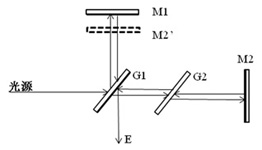
\includegraphics[width=0.55\linewidth]{g1.jpg}
			\caption{图1：迈克耳逊干涉仪的结构与光路图}
			\label{fig:structure}
		\end{figure}
		G1、G2 为材料、厚度相同的平行板，G1的一面镀上半反射膜，M1和M2为平面反射镜，M2是固定的，M1与精密丝杆相连，可以前后移动。M1和M2后各有三个小螺丝调节其方位。 
	
		光源S发出的光射向G1板而分成强度近似相等的两部分：反射部分1射到M1，经M1反射后再次透过G1进入接收器；透射部分2射到M2，经M2反射后再经 AG1的半反射膜反射到眼睛。这两束相干光束中各光线光程差不同，它们相遇时产生一定的干涉图样。
		
		为了使入射光线具有各种倾角，光源是扩展的。玻璃板G2起到补偿光程的作用：反射光束1通过玻璃板G1前后共三次，而透射光束2 只通过G1一次；有了G2，透射光束将往返通过它两次，从而使两束光在玻璃介质中的光程完全相等。如果光源是单色的，补偿与否无关紧要，但在使用白光时，就非有补偿板不可了。
		
		本实验中使用的He-Ne激光器单色性良好。
		
		\item \textbf{测量激光波长的原理}
		
		记M'2为M2在M1方向上的等效反射位置，氦氖激光器S发出的光束经干涉仪等效薄膜表面M1和M'2反射后，可视作激光产生薄膜干涉。记M1与M'2距离为 $d$，则在干涉条纹中心光程差为 $2d$；只要M1和 M'2足够大，在点光源同侧的任一点上，总能有相干光线相交，从而在E处可观察到干涉现象，因而这种干涉是非定域的。

		M1 和 M'2 之间的距离每改变 $\frac{\lambda}2$，干涉条纹中心就“产生”或“消失”一个圆环，同时条纹之间的间隔（即条纹的稀疏）也发生变化。因此吞吐干涉条纹个数 $n$、光程差 $2d$ 和波长 $\lambda$ 有关系：
		
		$$ 2\Delta d = \dfrac{\lambda}{n}$$

		可得

		$$\lambda = \frac{2\Delta d}{n}$$

		\item \textbf{逐差法数据处理}
		
		为提高测量精度，本实验采用逐差法处理数据：一次调节 M1 令中心条纹连续变化 $n=50$ 条；重复测量 $12$ 组。计算波长时，取  
		$$
		\Delta d_i = d_{i+6}-d_i \quad(i=1,2,\dots,6),
		$$
		并对所有 $\Delta d_i$ 取平均，有

		\begin{align*}
		\lambda &= \frac{2}{50} \times \frac{(d_{7}-d_{1})+(d_{8}-d_{2})+(d_{9}-d_{3})+(d_{10}-d_{4})+(d_{11}-d_{5})+(d_{12}-d_{6})}{6 \times 6} \\
		&= \frac{2}{50} \times \frac{\Delta d_1 + \Delta d_2 + \Delta d_3 + \Delta d_4 + \Delta d_5 + \Delta d_6}{6 \times 6}
		\end{align*}
		
	\end{enumerate}
	
	\section*{\textbf{{四. 实验仪器}}}
	迈克尔逊干涉仪，氦氖激光器，短焦透镜

	\section*{\textbf{{五. 实验内容}}}

	\begin{enumerate}
		\item 启动氦氖激光器，调节激光器的朝向和高度使激光在分束器上的入射角为$45^{\circ}$，此时光源到M1的逆光路与原光路重合。调节M1、M2后部的三支调节螺钉，使两束反射光的最亮光点在毛玻璃屏上重合为一个光点。
		\item 在激光器和分束器间插入短焦距透镜以形成扩展源，调整透镜朝向高度使各光学器件共轴，此时屏幕出现以光轴为圆心的同心圆干涉条纹。
		\item 缓慢转动鼓轮改变M1的位置，每出现（或消失）$n=50$ 条纹时读取一次示数 $d_i$；特殊地，$d_1$为开始转动前的初始示数。观察条纹疏密变化与同心圆中心“吞吐”现象。
		\item \textbf{连续}记录 $12$ 组读数 $\{d_1,d_2,\dots,d_{12}\}$。
		\item 根据测量数据计算氦氖激光器波长。
	
	\end{enumerate}
	\section*{\textbf{{六. 数据记录}}}
	
	原始测量数据见附表 1。

	\section*{\textbf{{七. 数据处理}}}

	\begin{enumerate}
		
	\item \textbf{根据测量数据计算氦氖激光波长}
	
	根据测量数据计算得到逐差 $\Delta d_i = d_{i+6}-d_i$，如附表 1 所示。
	
	\begin{table}[H]
		\centering
		\renewcommand{\arraystretch}{1.3} % 调整行距，1.3 为示例，可根据需要调整
		\begin{tabular}{|c|c|c|c|c|c|}
			\hline
			$\Delta d_1$     & $\Delta d_2$     & $\Delta d_3$     & $\Delta d_4$     & $\Delta d_5$     & $\Delta d_6$  \\ \hline
			0.09500mm  &   0.09550mm  & 0.09481mm  & 0.09568mm  & 0.09510mm & 0.09529mm  \\ \hline
		\end{tabular}
		\caption{氦氖激光器波长测量数据逐差表} % 添加表格标题
		\label{tab:wave_length_data} % 添加引用标签
	\end{table}

	有逐差平均值 $\bar{\Delta d} = 0.09523$mm

	则氦氖激光器波长为
	
	\begin{align*}
		\lambda &=\frac{2}{50} \times \frac{\Delta d_1 + \Delta d_2 + \Delta d_3 + \Delta d_4 + \Delta d_5 + \Delta d_6}{6 \times 6} \\
		&=\frac{2}{50}\times\frac{0.09500+0.09550+0.09481+0.09568+0.09510+0.09529}{6\times 6}\mathrm{mm} \\
		&=634.87\mathrm{nm}
	\end{align*}
	
	\item \textbf{计算不确定度}
	
	A类不确定度：

\begin{equation}
	\begin{aligned}
		u_{A}({\Delta d})
		&=\sqrt{\frac{\sum_{i=1}^{6}\bigl(\Delta d_i-\overline{\Delta d}\bigr)^{2}}{6(6-1)}} \\
		&=\sqrt{\frac{%
				\begin{aligned}
					& (0.09500-0.09523)^{2}+(0.09550-0.09523)^{2}\\
					&+(0.09481-0.09523)^{2}+(0.09568-0.09523)^{2}\\
					&+(0.09510-0.09523)^{2}+(0.09529-0.09523)^{2}
			\end{aligned}}
			{30}} \\[8pt]
		&\approx 7.8468\times10^{-5}\ \text{mm} = 78.468\text{nm}.
	\end{aligned}
\end{equation}
	
	\textbf{B类不确定度：}

	仪器的最小刻度为

	$$\frac{\text{标尺最小分度}}{\text{粗调手轮刻度数}\times\text{细调手轮刻度数}} = \frac{1\mathrm{mm}}{100\times 100} = 100\mathrm{nm}$$
	\\
	则仪器的最大允差为：
	\[ 
	\Delta_{\text{仪}}\approx100\mathrm{nm}
	 \]
	 由于逐差法得到的$\Delta d$需要读数两次，其等效最大允差为：
	 \[ 
	 \Delta_{B} = \sqrt{\Delta_{\text{仪}}^2+\Delta_{\text{仪}}^2}=\sqrt{2}\Delta_{\text{仪}}
	 \]
	 测量仪器机构类似螺旋测微计，误差为正态分布，置信系数 $C = 3$，则 
	 $$u_{B}(\Delta D) = \dfrac{\sqrt{\Delta_B}}{C} = \dfrac{\sqrt{2} \times 100 \mathrm{nm}}{3} = 47.14\mathrm{nm}$$

	\textbf{各物理量在 $P = 0.95$ 时的合成不确定度：}
	
	$P=0.95$时：
	\begin{itemize}
		\item $n = 6$时的$t$因子$t_{0.95}=2.57$；
		\item 仪器误差视为正态分布，取$k_{0.95}=1.96$。
	\end{itemize}
	
	故：
	
	$$ u_{0.95}(\Delta d) = \sqrt{(t_{0.95}u_{A}(\Delta d))^{2}+(k_{0.95}u_{B}(\Delta d))^{2}} = \sqrt{(2.57\times 78.468)^2 + (1.96\times 47.14)^2} \approx 221.8\mathrm{nm}$$
	
	\textbf{波长的不确定度：}
	
	根据不确定度的传递公式：
	
	$$ u(\lambda) = \dfrac{2}{n}u(\Delta d) = \dfrac{2}{50}\times 221.8 = 8.873\mathrm{nm}$$
	
	\item \textbf{测量结果完整表达式}
	
	实验测得的氦氖激光波长 $\lambda = (634.87 \pm 8.873)\mathrm{nm}\quad (P=0.95)$.
	
	氦氖激光波长参考值632.8nm，则测量值的相对误差：
	$$ \frac{\Delta \lambda}{\lambda} = \frac{|634.87-632.8|}{632.8} \approx \times 0.327\% < 1\% $$

	误差在实验要求范围内。

	\end{enumerate}

	\section*{\textbf{八. 误差分析}}
	\begin{enumerate}
		\item 实验台振动等稳定性因素导致干涉条纹瞬时漂移，影响光程差稳定性。
		\item 观测到的干涉图样的波峰波谷并不明确，实验人员读数难以做到保证两次读数环带的位置完全一致，带来随机误差。
		\item $M_1,M_2$可能不完全平行，无法形成纯粹的等倾干涉，干涉图样出现畸变，波
		
		长和光程差的关系不再准确。
		\item 逐差法仅取 $6$ 组差值求平均，仍存在有限样本引起的统计方差。
		\item 仪器最小分度有限，读数主观估读导致 $\Delta d$ 的系统误差；
	\end{enumerate}

	\section*{\textbf{{九. 问题思考}}}

	\begin{enumerate}
		\item \textbf{分光板的作用是什么？若分光板存在微小倾斜，会对实验产生什么影响？}

		分光板使激光分为反射光与透射光，反射光射向$M_1$，透射光射向$M_2$；被两镜子反射的光又各自被一分为二，其中来自$M_1$的透射光和来自$M_2$的反射光将重合，且两束光将具有稳定的光程差，相同的频率和平行的振动分量（来自同一光源），在观察屏上形成稳定干涉条纹。  

		若分光板存在微小倾斜,则两束光路将不完全重合，圆形等倾干涉条纹可能变形为倾斜条纹或条纹对比度下降；条纹中心将偏移，导致理论光程差模型不再成立，从而在波长或其他参数的计算中引入系统误差。
		
		\item \textbf{如何利用迈克耳逊干涉仪测量透明薄膜的折射率？请简述实验思路。}
		
		调节迈克尔逊干涉仪使毛玻璃上稳定呈现同心圆条纹，记录此时圆心条纹状态。将厚度已知为 $t$ 的透明薄膜垂直插入其中一臂，初始与光路垂直。缓慢旋转薄膜至倾斜一定角度 $\theta$，记录此时圆心条纹状态的变化。继续旋转薄膜，每当圆心条纹“产生”或“消失” $N$ 条时，记录下此时的旋转角度 $\theta_N$。根据干涉条纹的变化计算光程差的变化 $\Delta d$，根据公式 $\Delta d = 2t(n-1)(1-\cos\theta_N)$ 可以计算出薄膜的折射率 $n$。
	\end{enumerate}

	
	\section*{\textbf{{十. 实验结论}}}
	
	本实验使用迈克尔逊干涉仪，测得氦氖激光波长 $g = (634.87 \pm 8.873)\mathrm{nm} \quad (P=0.95)$，相对误差为$0.327\% < 1\% $，在实验设计要求范围内。
	
	

\end{document}